\documentclass[10pt, a4paper]{article}
\usepackage[utf8]{inputenc}
\usepackage[a4paper, total={6in, 10in}]{geometry}

\title{WSM Project 2}
\author{Joanna Chien 106306035 MIS}
\date{May 2021}

\usepackage{natbib}
\usepackage{graphicx}
\usepackage{dirtree}
\usepackage{subfigure}

\begin{document}

\maketitle

\section{Abstract}
This experiment use Indri-5.18 to run the 50 TREC queries against WT2G collection, and evaluate the returned ranked list. The implemented ranking functions containing vector space model(Okapi TF $\times$ IDF), language model and some smoothing functions. Besides tuning ranking functions, I also modify the queries according to the TREC queries description and narrative.

This report will be divided into four part. In part one, I will introduce the environmental setups and compare 2 types of indexing methods, whether to use stemming and then whether to use stop words filtering. After choosing proper indexing method, I will discuss the impact of query types by running 3 different types of queries under same indexing method and ranking function. After comparing query types and indexing methods, this report will compare the result of different ranking functions to see which one of the ranking functions performs the best. For the final part, there will be the comparison among all settable parameters' combinations, to verify the assumption made by previous parts or determine which set of parameters' combination is suitable for what situation.

\section{Experiment Setup and Indexing Methods Comparison}
\label{section:2}
This section will introduce the basic setups of the experiment, including environmental setup, parameters setup when building index, and introduce the differences and parameters in running queries between different cases.

\subsection{Environmental Setup Steps and File Trees}
The operating system used is macOS Mojave 10.14.6. After downloading Indri-5.18, install \verb|gcc@6| through Homebrew. Then configure Indri project, modify \verb|MakeDefns| and \verb|atomic.hpp| file. After modifying these settings, run make install to install Indri to system.

The following shows the file tree of this experiment:

\dirtree{%
.1 Project2.
.2 indri{-}5{.}18.
.2 run.
.3 index.
.4 WT2G.
.4 WT2G$\_$stop.
.4 WT2G$\_$stemmer.
.4 WT2G$\_$stemmer$\_$stop.
.3 params.
.4 index.
.4 none.
.4 none$\_$stop.
.4 stemmer.
.4 stemmer$\_$stop.
.3 run{.}sh.
.3 trec$\_$eval.
.2 WT2G.
}

Like the file tree shows, there are 4 different indexing methods, including normal indexing, indexing with stop words filtering, indexing with stemmer, indexing with stemmer and stop words filtering.

\subsection{Indexing Methods Comparison}
\subsubsection{The Impact of Stemming}
In this part of experiment, I run the 50 TREC queries' title as query against WT2G collection with Okapi, Language Model(LM) and LM with JM smoothing function(LMJM) respectively, using both no stemming indexing and stemming indexing. 

\begin{figure}[h!]
\centering
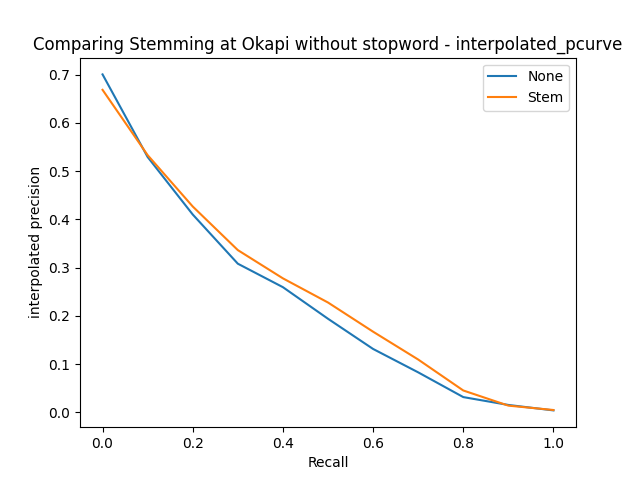
\includegraphics[scale=0.3]{compare stem/Comparing Stemming at Okapi without stopword - interpolated_pcurve-ipd.png}
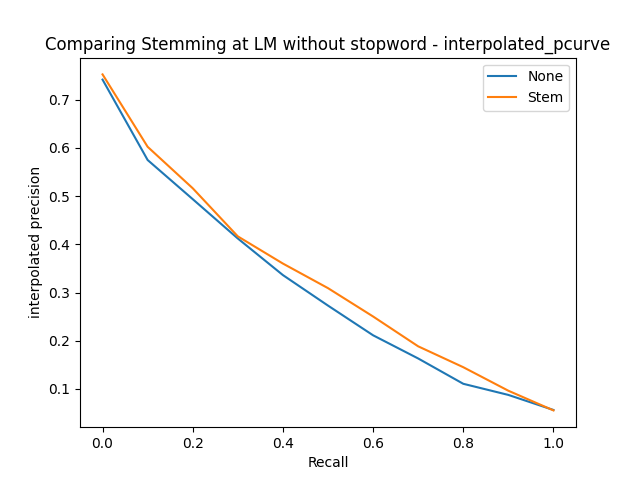
\includegraphics[scale=0.3]{compare stem/Comparing Stemming at LM without stopword - interpolated_pcurve-ipd.png}
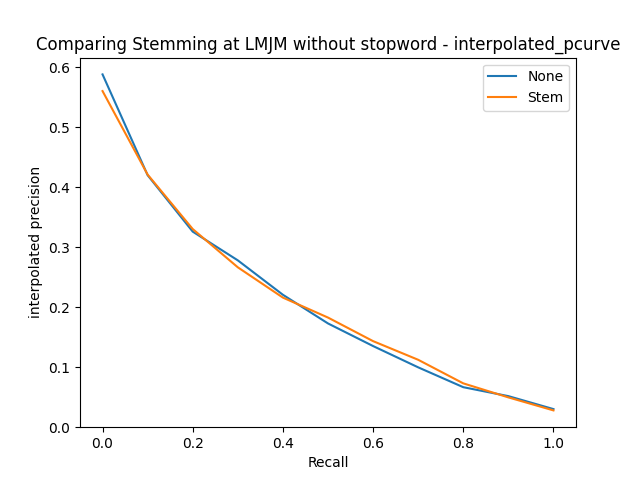
\includegraphics[scale=0.3]{compare stem/Comparing Stemming at LMJM without stopword - interpolated_pcurve-ipd.png}
\caption{Comparing Stemming at Okapi/LM/LMJM -- Interpolated Precision Curve}
\label{fig:stemming_i}
\end{figure}

In Figure \ref{fig:stemming_i}, we can observe that the precision without stemming indexing(blue line) is slightly higher than the precision with stemming indexing(orange line) at 0.1 recall level in both Okapi's and LMJM's cases. However, after 0.1 recall level, the precision with stemming indexing is stably higher than that of no stemming indexing result in Okapi's case. Furthermore, the precision with stemming indexing is also higher than precision of no stemming indexing at any recall level in LM's case. As for the LMJM's case, the two results of precision remains the same(with slight difference) at any recall level after 0.1.

\begin{figure}[h!]
\centering
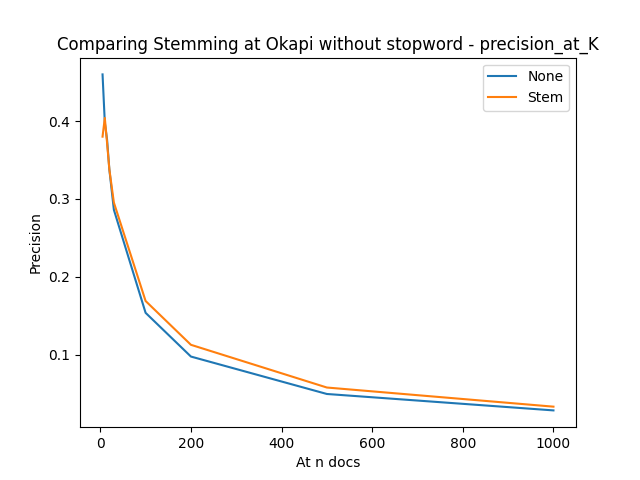
\includegraphics[scale=0.3]{compare stem/Comparing Stemming at Okapi without stopword - precision_at_K-pak.png}
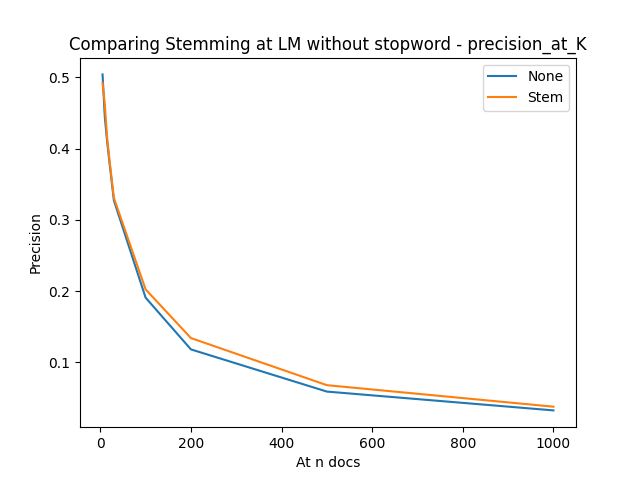
\includegraphics[scale=0.3]{compare stem/Comparing Stemming at LM without stopword - precision_at_K-pak.png}
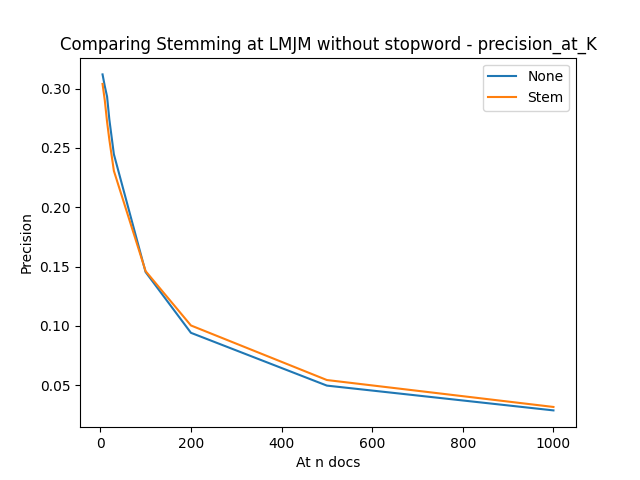
\includegraphics[scale=0.3]{compare stem/Comparing Stemming at LMJM without stopword - precision_at_K-pak.png}
\caption{Comparing Stemming at Okapi/LM/LMJM -- Precision at K}
\label{fig:stemming_p}
\end{figure}

Figure \ref{fig:stemming_p} shows the same result. Although the precision without stemming indexing is higher than that with stemming indexing in Okapi's case at first 5 documents, the precision with stemming indexing is slightly higher in most situation. Therefore, the retrieval system without stemming indexing is suitable for users who only care about first few retrieved results, while the retrieval system with stemming indexing is suitable for users who seeking for big amount of results, for the overall performance of this kind of system is better than the former one.

\begin{figure}[h!]
\centering
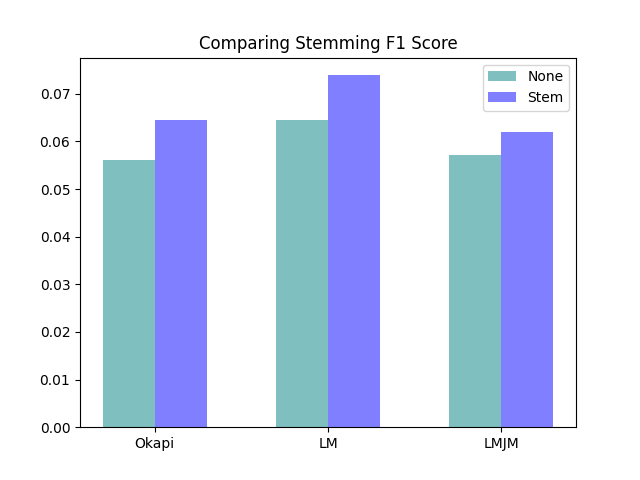
\includegraphics[scale=0.4]{compare stem/Comparing Stemming F1 Score.png}
\caption{Comparing Stemming at Okapi/LM/LMJM -- F1 score}
\label{fig:stemming_f}
\end{figure}
Figure \ref{fig:stemming_f} shows the F1 score under these two kinds of indexing method among three different cases. As we can see, the F1 score is better with stemming indexing than those without stemming indexing in all of the three cases.

In conclusion, with the help of stemming functions, the system could generalize and recognize more words more generally than the system without stemming. Consequently, the stemming system performs better than the system without stemming indexing.

\subsubsection{The Impact of Stop Words Filtering}
After measuring the importance of stemming indexing, this section will verify the impact of stop words filtering, to see if indexing with stop words filtering improves the system performance.
\begin{figure}[h!]
\centering
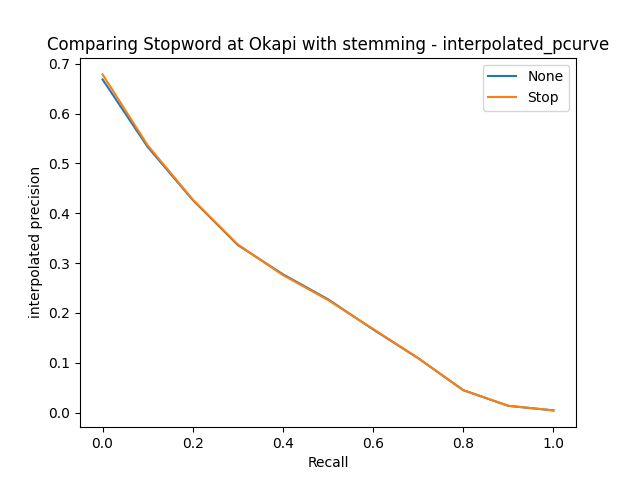
\includegraphics[scale=0.3]{compare stop/Comparing Stopword at Okapi with stemming - interpolated_pcurve-ipd.png}
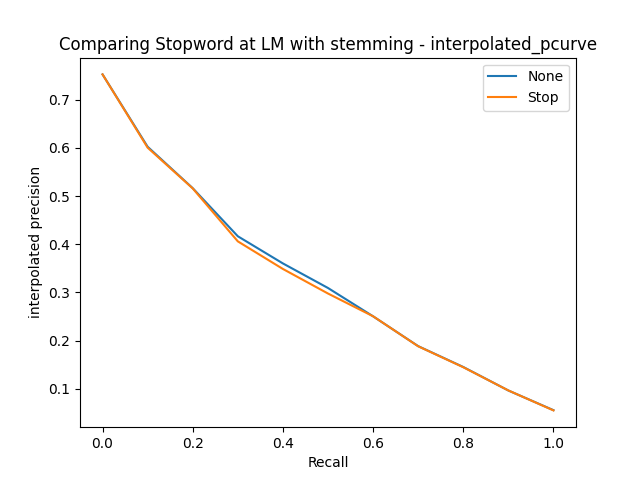
\includegraphics[scale=0.3]{compare stop/Comparing Stopword at LM with stemming - interpolated_pcurve-ipd.png}
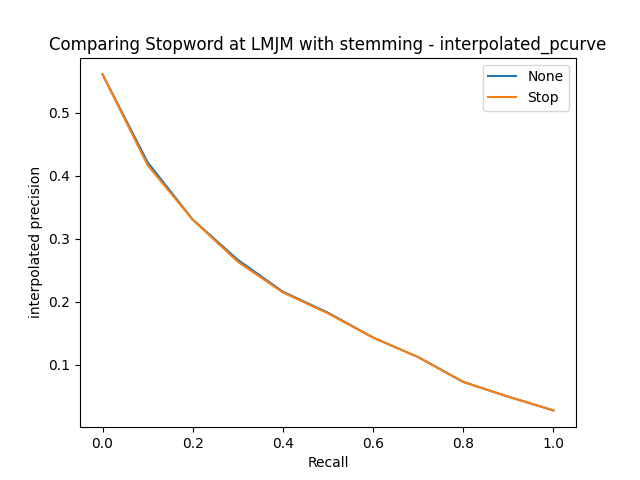
\includegraphics[scale=0.3]{compare stop/Comparing Stopword at LMJM with stemming - interpolated_pcurve-ipd.png}
\caption{Comparing Stop Words Filtering at Okapi/LM/LMJM -- Interpolated Precision Curve}
\label{fig:stop_i}
\end{figure}


\begin{figure}[h!]
\centering
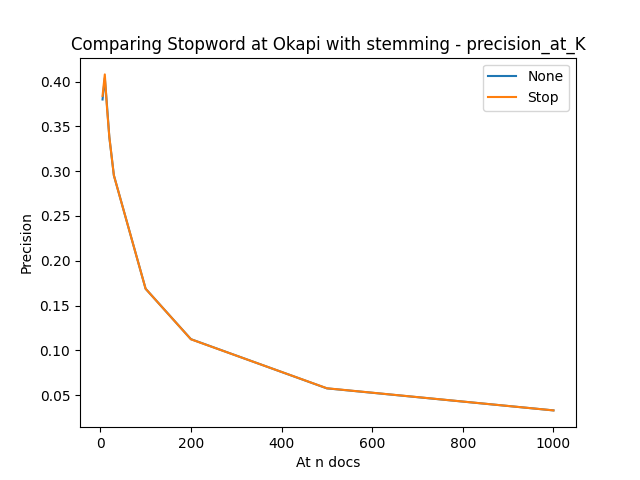
\includegraphics[scale=0.3]{compare stop/Comparing Stopword at Okapi with stemming - precision_at_K-pak.png}
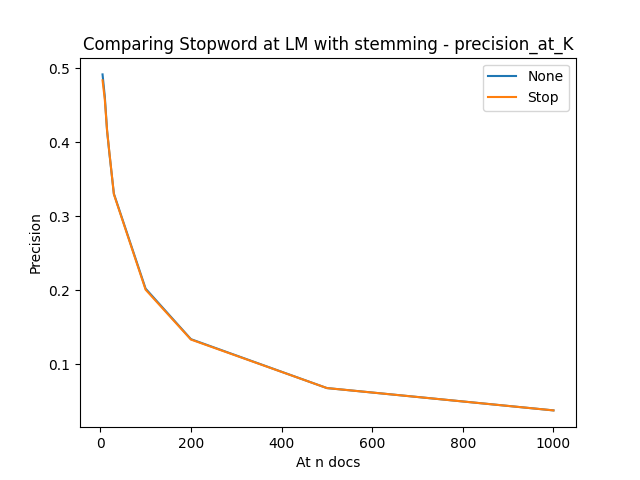
\includegraphics[scale=0.3]{compare stop/Comparing Stopword at LM with stemming - precision_at_K-pak.png}
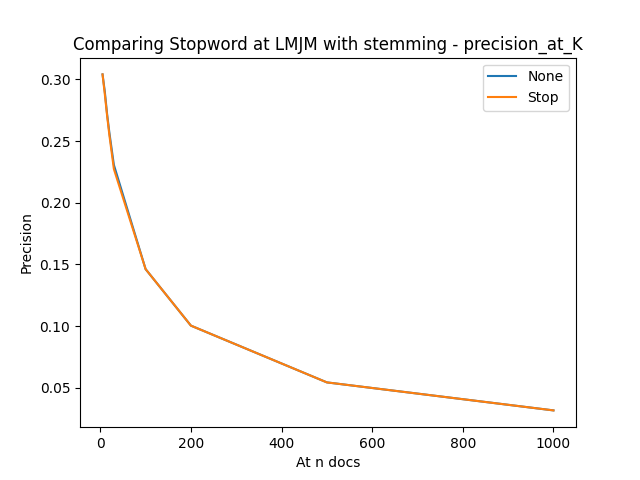
\includegraphics[scale=0.3]{compare stop/Comparing Stopword at LMJM with stemming - precision_at_K-pak.png}
\caption{Comparing Stop Words Filtering at Okapi/LM/LMJM -- Precision at K}
\label{fig:stop_p}
\end{figure}

\begin{figure}[h!]
\centering
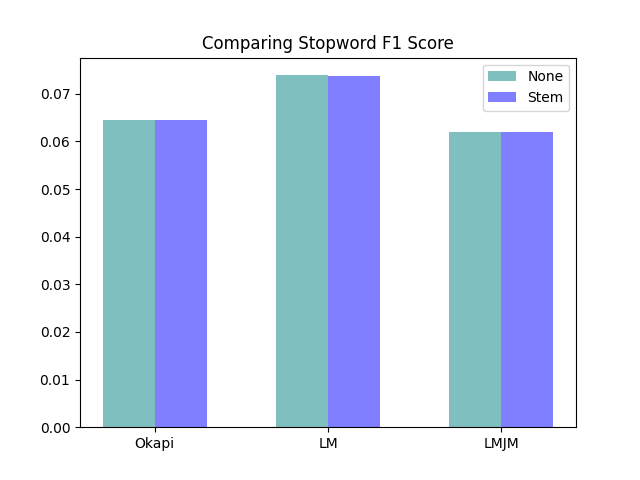
\includegraphics[scale=0.4]{compare stop/Comparing Stopword F1 Score.png}
\caption{Comparing Stop Words Filtering at Okapi/LM/LMJM -- F1 score}
\label{fig:stop_f}
\end{figure}

In both of Figure \ref{fig:stop_i} and Figure \ref{fig:stop_p}, the result precision of stop words filtering and no stop words filtering have almost no difference in both interpolated precision curve and precision at k curve. The only difference between the precision of these two indexing method(with/without stop words filtering) is in LM's case, where the precision of no stop words filtering indexing at about 0.2 to 0.6 recall level is slightly greater than those with stop words filtering in the interpolated precision curve. In the precision at k curve, there is merely no difference between two indexing methods. For this circumstance, I think the reason why systems perform very similarly is that the IDF function works similar to stop words filtering, and each one of these three ranking methods contains functions that works similar to IDF function, which causes both the system with and without stop words filtering show similar result.

In Figure \ref{fig:stop_f}, however, the F1 score shows that the performance of no stop words filtering is slightly better than those with stop words filtering. Therefore, in the following experiments, the indexing methods will be "indexing with stemming but without stop words filtering"




\section{Query Types Comparison}
\label{section:3}
After determining the parameters of indexing method, this section will discuss the impact of different type of queries. There are 3 types of queries in this section, which are "Normal", "Description" and "Description with title".

In the Normal's case, the queries used for retrieving documents only contains contents of the title tag in the TREC queries. As for the Description case, the queries for retrieval contains the descriptions tag's content, with stop words removal. Finally, the Description with title's case's queries combine the previous two cases, which means the queries of this case contain queries' title and description(with stop words filtering) from TREC queries.

\begin{figure}[h!]
\centering
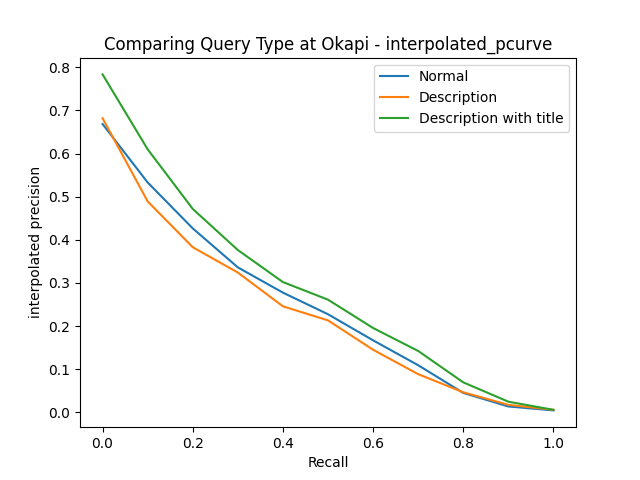
\includegraphics[scale=0.3]{compare query/Comparing Query Type at Okapi - interpolated_pcurve-ipd.png}
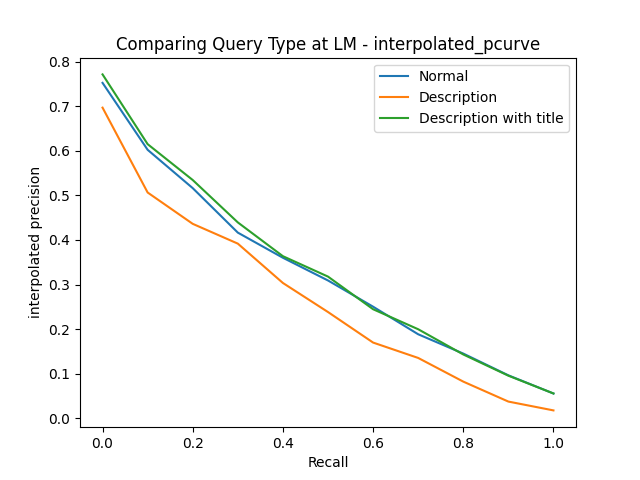
\includegraphics[scale=0.3]{compare query/Comparing Query Type at LM - interpolated_pcurve-ipd.png}
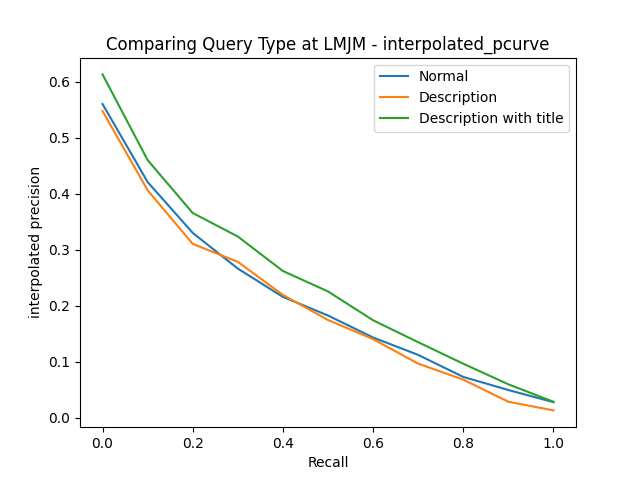
\includegraphics[scale=0.3]{compare query/Comparing Query Type at LMJM - interpolated_pcurve-ipd.png}
\caption{Comparing Query Types at Okapi/LM/LMJM --Interpolated Precision Curve}
\label{fig:q_i}
\end{figure}

In Figure \ref{fig:q_i}, we can see that the green curve(Description with title's case) outperform the other two curves under both Okapi and LMJM ranking functions, and the blue curve(Normal's case) performs similar to green curve under LM ranking function. The Description's case performs the worst among these three different query type.

\begin{figure}[h!]
\centering
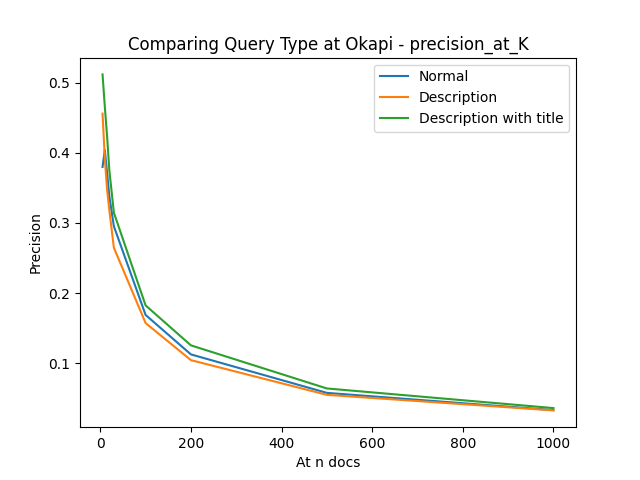
\includegraphics[scale=0.3]{compare query/Comparing Query Type at Okapi - precision_at_K-pak.png}
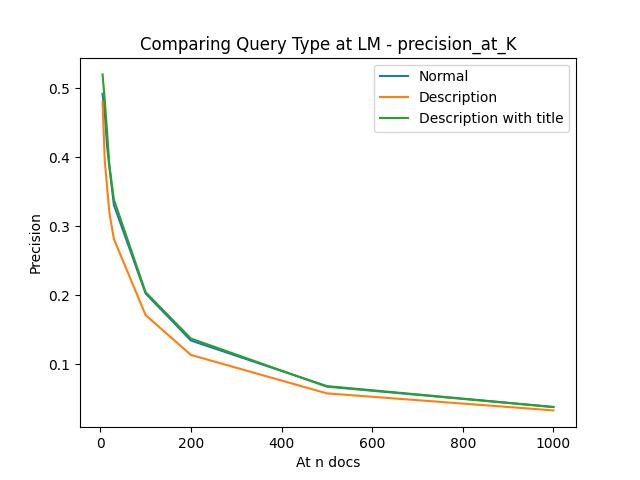
\includegraphics[scale=0.3]{compare query/Comparing Query Type at LM - precision_at_K-pak.png}
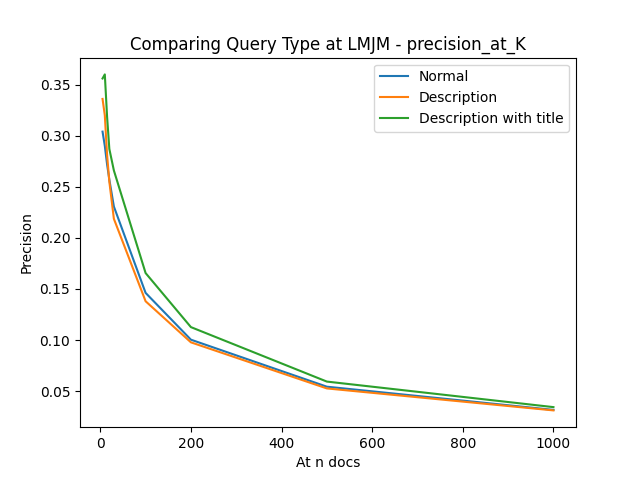
\includegraphics[scale=0.3]{compare query/Comparing Query Type at LMJM - precision_at_K-pak.png}
\caption{Comparing Query Types at Okapi/LM/LMJM -- Precision at K}
\label{fig:q_p}
\end{figure}

\begin{figure}[h!]
\centering
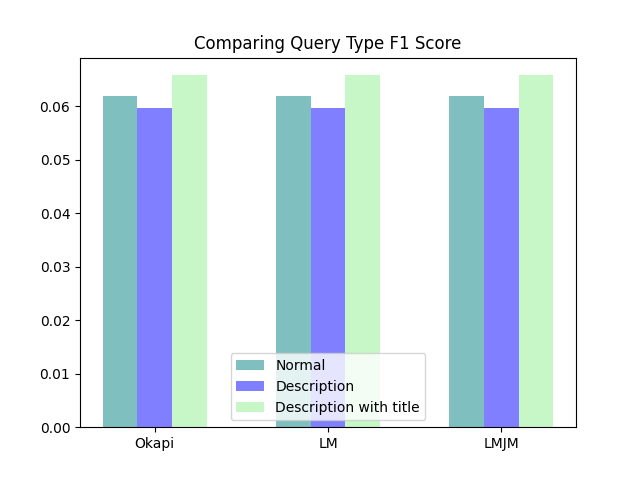
\includegraphics[scale=0.4]{compare query/Comparing Query Type F1 Score.png}
\caption{Comparing Query Types at Okapi/LM/LMJM -- Precision at KF1 score}
\label{fig:q_f}
\end{figure}

Figure \ref{fig:q_p} shows the same result. Although these three curves are very close to each other, we still can observe that the orange curve(Description's case) is in the leftmost of the figure, and the green curve(Description with title's case) always lies in the rightmost of the figure. To observe in a more general viewpoint, Figure \ref{fig:q_f} shows that the F1 of Description with title's case is higher than that of other two cases under every ranking functions.

There are two possible drawbacks of other two cases so that the Description with title case perform better than the other two cases. The first is that the Normal case contains too little information about the information needed by user. Another drawback for Description case is the content in description might not be specific enough for system to retrieve corresponding documents. However, the Description with title case combine title and description to make the query more specific and contains more hints about the information needs. Therefore, due to the better performance of the Description with title case, the query types used to measure ranking functions will be "Description with title" in the following sections.

\section{Ranking Functions Comparison}
\label{section:4}
\subsection{Comparing Okapi, LM and LMJM}
This section will discuss the performance of required 3 different ranking functions, including Okapi, Language Model and Language Model with JM smoothing function, to determine which one of these functions performs the best.


\begin{figure}[h!]
\centering    %居中
\subfigure[Comparing Ranking Functions --Interpolated Precision Curve] %第一張子圖
{
	\begin{minipage}{7cm}
	\centering          %子圖居中
	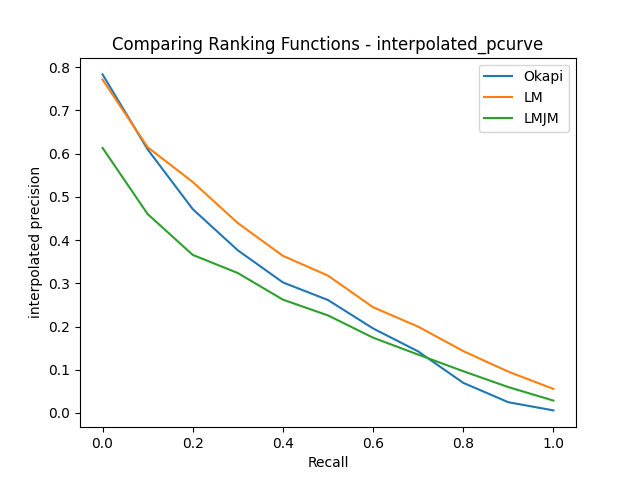
\includegraphics[scale=0.45]{compare ranking/Comparing Ranking Functions - interpolated_pcurve-ipd.png}
	\end{minipage}
}
\subfigure[Comparing Ranking Functions -- Precision at K] %第二張子圖
{
	\begin{minipage}{7cm}
	\centering      %子圖居中
	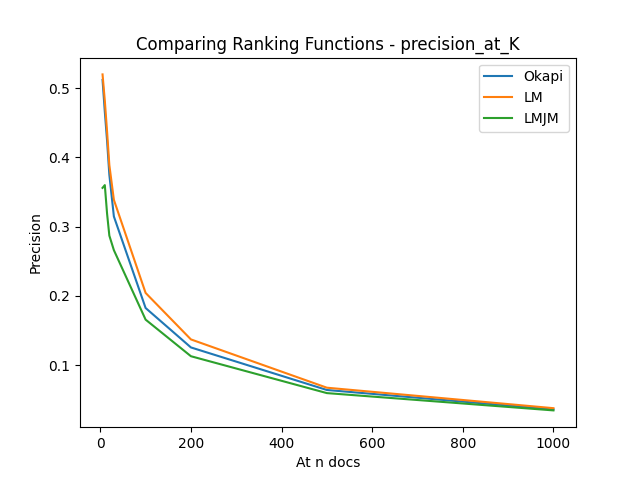
\includegraphics[scale=0.45]{compare ranking/Comparing Ranking Functions - precision_at_K-pak.png}
	\end{minipage}
}
\caption{Comparing Ranking Functions} %  %大圖名稱
\label{fig:r_ip}  %圖片引用標記
\end{figure}

According to the interpolated precision curve showed in Figure \ref{fig:r_ip}, the orange curve(LM case) possesses the highest precision at any given recall level and any amount of document retrieved in precision at k curve. As for other two cases, the Okapi function(blue curve) has higher precision at anterior results and close to the performance of LM system in both figure in Figure \ref{fig:r_ip} which makes it suitable for users who focus on top results. Furthermore, the performance of Okapi function even surpass that of LM function in the Interpolated precision curve before 0.1 recall level. However, the LMJM function performs not very well in the both graph in Figure \ref{fig:r_ip}. The precision of LMJM case only surpass Okapi's after 0.7 recall level,  making the overall results retrieved by LMJM might be slightly better than Okapi's overall results.


\begin{figure}[h!]
\centering
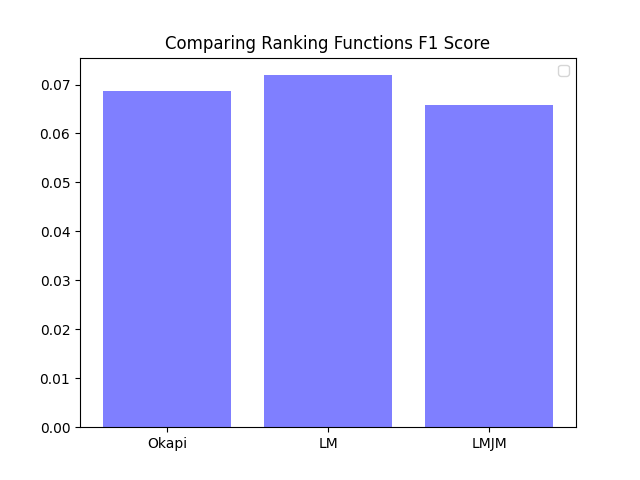
\includegraphics[scale=0.5]{compare ranking/Comparing Ranking Functions F1 Score.png}
\caption{Comparing Ranking Functions -- F1 score}
\label{fig:r_f}
\end{figure}

Figure \ref{fig:r_f} shows the same results. LM case's F1 score is obviously higher than the other two ranking methods, and Okapi's F1 score is also slightly higher than LMJM's. The possible reason is that the lambda of JM smoothing might not be optimal, therefore causing the result worse than the LM without JM smoothing one. Additionally, we can see that the performance of query generation(language model) is better than the performance of document generation(Okapi).


\subsection{Add Pseudo Feedback}

After figuring out the best ranking function is LM among the basic required 3 functions, I decided to add pseudo feedback to the LM ranking function(LMFB) to see if the result is better than all of the three basic required ranking functions.

\begin{figure}[h!]
\centering    %居中
\subfigure[Comparing Ranking Functions(add LMFB) --Interpolated Precision Curve] %第一張子圖
{
	\begin{minipage}{7cm}
	\centering          %子圖居中
	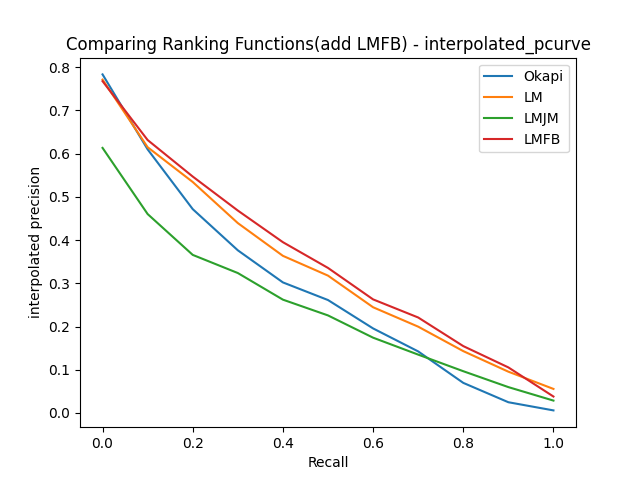
\includegraphics[scale=0.45]{add LMFB/Comparing Ranking Functions(add LMFB) - interpolated_pcurve-ipd.png}
	\end{minipage}
}
\subfigure[Comparing Ranking Functions(add LMFB) -- Precision at K] %第二張子圖
{
	\begin{minipage}{7cm}
	\centering      %子圖居中
	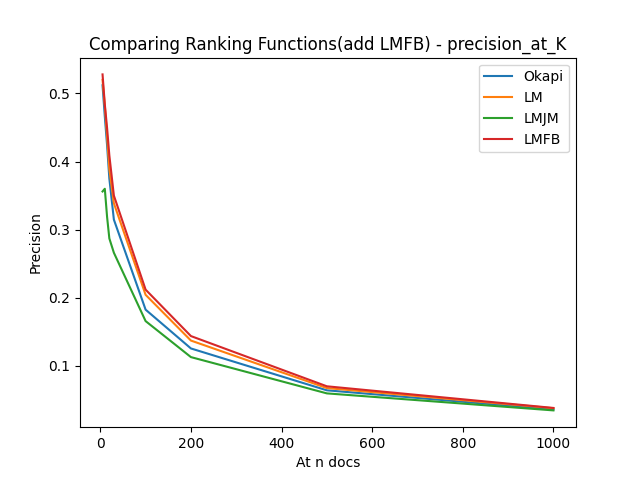
\includegraphics[scale=0.45]{add LMFB/Comparing Ranking Functions(add LMFB) - precision_at_K-pak.png}
	\end{minipage}
}
\caption{Comparing Ranking Functions(add LMFB)} %  %大圖名稱
\label{fig:fb_ip}  %圖片引用標記
\end{figure}

As the result precision showed in Figure \ref{fig:fb_ip}, we can see that the LM with pseudo feedback(LMFB, red curve) performs almost the same as the LM's performance(orange curve), but even slightly better than LM. Only at about 0.9 recall level does the red curve lower than the orange curve. However, the Okapi's performance(blue curve) is still better than the LMFB's before but only at 0.1 recall level. For the precision at k curve in Figure \ref{fig:fb_ip}, although the red curve and orange curve are very close to each other, we can still see that red curve slightly greater than the orange curve at 50~500 documents.

\begin{figure}[h!]
\centering
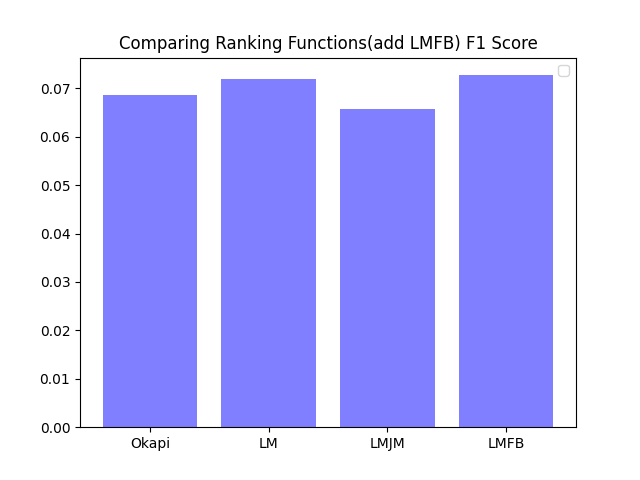
\includegraphics[scale=0.5]{add LMFB/Comparing Ranking Functions(add LMFB) F1 Score.png}
\caption{Comparing Ranking Functions(add LMFB) -- F1 score}
\label{fig:fb_f}
\end{figure}

For the F1 score of the LMFB's case, the score is 0.0727, which is very close to LM's case whose score is 0.0719, which also shows that the LMFB's case is the best ranking function among these four ranking methods. The possible reason is that, since the LM's case is already the better ranking function among the three required functions, adding the pseudo feedback according to LM's result to tune the result could definitely help the system to retrieve document more precisely.

To sum up, the current best retrieval method is indexing with stemming, query with description and title, and ranking with language model and its pseudo feedback.

\section{Comparing All Retrieved Results}
\label{section:5}
In this section, I run all the possible parameters combinations, and sort each retrieval methods in terms of F1 score, precision score, recall score and average precision. Through the comparison in this section, I will verify the assumptions made in previous sections are correct or not. This section will be divided into 4 parts for each corresponding sorting basis.

\subsection{Methods Sorted by F1 score}

\begin{center}
\begin{tabular}{ |c|c|c|c|c|c|c|c|c|c|c| } 
\hline
method_i  & index & stop & rank$\_$fn & query & f1 & precision & recall & AP \\
\hline
 9 & Stem & none & LM & Normal & 0.0739 &  0.0387 & 0.8293 & 0.3113 \\ 
13 & Stem & Stop & LM & Normal & 0.0738 &  0.0386 & 0.8284 & 0.3079 \\ 
47 & Stem & Stop & LMFB &  q+des & 0.0735 &  0.0384 & 0.8425 & 0.3250 \\ 
15 & Stem & Stop & LMFB & Normal & 0.0731 &  0.0382 & 0.8381 & 0.3288 \\ 
43 & Stem & none & LMFB &  q+des & 0.0727 &  0.0380 & 0.8328 & 0.3307 \\ 
11 & Stem & none & LMFB & Normal & 0.0727 &  0.0380 & 0.8337 & 0.3260 \\ 
41 & Stem & none & LM &  q+des & 0.0719 &  0.0376 & 0.8240 & 0.3160 \\ 
45 & Stem & Stop & LM &  q+des & 0.0717 &  0.0375 & 0.8227 & 0.3125 \\ 
44 & Stem & Stop &  Okapi &  q+des & 0.0687 &  0.0359 & 0.7872 & 0.2697 \\ 
40 & Stem & none &  Okapi &  q+des & 0.0687 &  0.0359 & 0.7872 & 0.2688 \\ 
\hline
\end{tabular}
\end{center}

\begin{center}
\begin{tabular}{|l|l|l|l|l|l|l|l|l|}
\hline
\multicolumn{2}{|l|}{Indexing Methods} & \multicolumn{4}{l|}{Ranking Functions} & \multicolumn{3}{l|}{Query Types}              \\ \hline
Stem               & Stop              & Okapi     & LM     & LMJM    & LMFB    & Normal & Description & Description with title \\ \hline
9                  & 6                 & 2         & 4      & 0       & 4       & 4      & 0           & 6                      \\ \hline
\end{tabular}
\end{center}

As mentioned above, we can learn that the indexing with stemming is important from the table above, among ten best 10 ranking methods, there are 9 of them use stemming indexing, and the result remains the same in the following records. However, there are two difference between this result and the previous assumptions. For the first one difference, in the perspective of F1 score, the LM ranking function performs slightly better than the LMFB ranking method, but the Okapi ranking function remains the same performance. For the second difference, the best few methods use the Normal query, but the Description with title query type still appears more in the whole 10 best methods.

As a result, if the user requires both precision and recall score high enough, then the system should use stemming indexing without stop words filtering, query the collection with Normal queries, and rank the results with LM ranking function just like method_9.

\subsection{Methods Sorted by Precision Score}
\begin{center}
\begin{tabular}{ |c|c|c|c|c|c|c|c|c|c|c| } 
\hline
method_i  & index & stop & rank$\_$fn & query & f1 & precision & recall & AP \\
\hline
9 & Stem & none & LM & Normal & 0.0739 &  0.0387 & 0.8293 & 0.3113 \\
 13 & Stem & Stop & LM & Normal & 0.0738 &  0.0386 & 0.8284 & 0.3079 \\
 47 & Stem & Stop & LMFB &  q+des & 0.0735 &  0.0384 & 0.8425 & 0.3250 \\
 15 & Stem & Stop & LMFB & Normal & 0.0731 &  0.0382 & 0.8381 & 0.3288 \\
 43 & Stem & none & LMFB &  q+des & 0.0727 &  0.0380 & 0.8328 & 0.3307 \\
 11 & Stem & none & LMFB & Normal & 0.0727 &  0.0380 & 0.8337 & 0.3260 \\
 41 & Stem & none & LM &  q+des & 0.0719 &  0.0376 & 0.8240 & 0.3160 \\
 45 & Stem & Stop & LM &  q+des & 0.0717 &  0.0375 & 0.8227 & 0.3125 \\
 44 & Stem & Stop &  Okapi &  q+des & 0.0687 &  0.0359 & 0.7872 & 0.2697 \\
 40 & Stem & none &  Okapi &  q+des & 0.0687 &  0.0359 & 0.7872 & 0.2688 \\
\hline
\end{tabular}
\end{center}

\begin{center}
\begin{tabular}{|l|l|l|l|l|l|l|l|l|}
\hline
\multicolumn{2}{|l|}{Indexing Methods} & \multicolumn{4}{l|}{Ranking Functions} & \multicolumn{3}{l|}{Query Types}              \\ \hline
Stem               & Stop              & Okapi     & LM     & LMJM    & LMFB    & Normal & Description & Description with title \\ \hline
10                  & 5                 & 2         & 4      & 0       & 4       & 4      & 0           & 6                      \\ \hline
\end{tabular}
\end{center}

The methods sorted by precision score is similar to the result of sorting by F1 score. It is because the F1 score will punish the lower score between precision and recall, and the precision is much lower than the recall score on average. Similarly, if the user requires higher precision of the results, or the system is used in trash main filtering etc., the system should also possess the parameters same as method_9 as well.

\subsection{Methods Sorted by Recall Score}
\begin{center}
\begin{tabular}{ |c|c|c|c|c|c|c|c|c|c|c| } 
\hline
method_i  & index & stop & rank$\_$fn & query & f1 & precision & recall & AP \\
\hline
 47 & Stem & Stop & LMFB &  q+des & 0.0735 &  0.0384 & 0.8425 & 0.3250 \\
 15 & Stem & Stop & LMFB & Normal & 0.0731 &  0.0382 & 0.8381 & 0.3288 \\
 11 & Stem & none & LMFB & Normal & 0.0727 &  0.0380 & 0.8337 & 0.3260 \\
 43 & Stem & none & LMFB &  q+des & 0.0727 &  0.0380 & 0.8328 & 0.3307 \\
9 & Stem & none & LM & Normal & 0.0739 &  0.0387 & 0.8293 & 0.3113 \\
 13 & Stem & Stop & LM & Normal & 0.0738 &  0.0386 & 0.8284 & 0.3079 \\
 41 & Stem & none & LM &  q+des & 0.0719 &  0.0376 & 0.8240 & 0.3160 \\
 45 & Stem & Stop & LM &  q+des & 0.0717 &  0.0375 & 0.8227 & 0.3125 \\
 44 & Stem & Stop &  Okapi &  q+des & 0.0687 &  0.0359 & 0.7872 & 0.2697 \\
 40 & Stem & none &  Okapi &  q+des & 0.0687 &  0.0359 & 0.7872 & 0.2688 \\
\hline
\end{tabular}
\end{center}

\begin{center}
\begin{tabular}{|l|l|l|l|l|l|l|l|l|}
\hline
\multicolumn{2}{|l|}{Indexing Methods} & \multicolumn{4}{l|}{Ranking Functions} & \multicolumn{3}{l|}{Query Types}              \\ \hline
Stem               & Stop              & Okapi     & LM     & LMJM    & LMFB    & Normal & Description & Description with title \\ \hline
10                  & 5                 & 2         & 4      & 0       & 4       & 4      & 0           & 6                      \\ \hline
\end{tabular}
\end{center}

In the methods sorted by recall score, the best method with highest recall value use almost the same as the assumption made in previous sections, except for the indexing method contains stop words filtering. All of the best 10 methods use stemming indexing in terms with recall score, and top 4 best methods use LMFB as ranking function. Furthermore, according to the table above, we can also determine the relationship among the four ranking functions is LMFB $>$ LM $>$ Okapi $>$ LMJM. Additionally, in the aspect of query types, the Description with title case provide more stable performance than Normal case's on average.

As a result, the best method is method$_{47}$ in terms of recall score, which has highest recall score and third highest precision score, making this method very suitable for searching documnets.

\subsection{Methods Sorted by Average Precision Score}
\begin{center}
\begin{tabular}{ |c|c|c|c|c|c|c|c|c|c| } 
\hline
method_i  & index & stop & rank$\_$fn & query & f1 & precision & recall & AP \\
\hline
 43 & Stem & none & LMFB &  q+des & 0.0727 &  0.0380 & 0.8328 & 0.3307  \\
 15 & Stem & Stop & LMFB & Normal & 0.0731 &  0.0382 & 0.8381 & 0.3288  \\
 11 & Stem & none & LMFB & Normal & 0.0727 &  0.0380 & 0.8337 & 0.3260  \\
 47 & Stem & Stop & LMFB &  q+des & 0.0735 &  0.0384 & 0.8425 & 0.3250 \\
 39 & none & Stop & LMFB &  q+des & 0.0668 &  0.0349 & 0.7657 & 0.3204  \\
 41 & Stem & none & LM &  q+des & 0.0719 &  0.0376 & 0.8240 & 0.3160  \\
7 & none & Stop & LMFB & Normal & 0.0662 &  0.0346 & 0.7582 & 0.3154 \\
 45 & Stem & Stop & LM &  q+des & 0.0717 &  0.0375 & 0.8227 & 0.3125  \\
9 & Stem & none & LM & Normal & 0.0739 &  0.0387 & 0.8293 & 0.3113 \\
 13 & Stem & Stop & LM & Normal & 0.0738 &  0.0386 & 0.8284 & 0.3079  \\
\hline
\end{tabular}
\end{center}

\begin{center}
\begin{tabular}{|l|l|l|l|l|l|l|l|l|}
\hline
\multicolumn{2}{|l|}{Indexing Methods} & \multicolumn{4}{l|}{Ranking Functions} & \multicolumn{3}{l|}{Query Types}              \\ \hline
Stem               & Stop              & Okapi     & LM     & LMJM    & LMFB    & Normal & Description & Description with title \\ \hline
8                  & 6                 & 0         & 4      & 0       & 6       & 5      & 0           & 5                      \\ \hline
\end{tabular}
\end{center}

In the perspective of average precision, the best parameter combination method$_{43}$ use exactly the same assumption in the previous sections(Section \ref{section:2} through Section \ref{section:4}). The possible reason is that, the average precision is the indicators that reflect global effectiveness, and I always choose the rightmost curve in the interpolated precision curve and precision at k curve in the previous sections. Therefore, the previous assumptions are consistent with average precision score, showing that method$_{43}$ possess the best performance on overall retrieval results.

\section{Conclusion}

In Section \ref{section:2}, it is determined that the stemming is important as an indexing function, but stop words filtering might not be as necessary as stemming due to the IDF implied functions in ranking methods. As for query types in Section \ref{section:3}, we learned that the normal query title in TREC queries might be sufficient enough to retrieve documents. However, with the help of the description of the query without stop words, the result precision score increase in most of the cases. As for the ranking functions in Section \ref{section:4}, the LM's function always out performance to other functions, and the results are even better when added pseudo feedback to LM ranking function.

Through Section \ref{section:2} to \ref{section:4}, we determined the best retrieving function in the aspect of interpolated precision curve and precision at k curve. However, there is still some other indicators that is not taken in the previous sections. Therefore, Section \ref{section:5} shows all different parameter combinations and explain which combination is suitable for each indicators. For F1 and precision score, the system should use stemming indexing without stop words filtering, query the collection with normal queries, and ran the results with LM ranking function. For recall score, the method with stemming indexing with stop words filtering, query with Description with title type query, and rank results with LMFB function possess the highest recall value, making it the best method for searching documents. For the aspect of average precision, the best retrieving method is the same as the assumption made in Section \ref{section:2} to Section \ref{section:4}, because they both observed in the same view point.
 
As for the further research of this project, I think there are some parameter which is able to be tuned in the future, such as lambda in JM smoothing, other types of queries and some other ranking functions. Through this project, I learned more about how to evaluate the retrieving functions, and how to draw corresponding data graphs. This project also helps me clarify the difference between the indicators and the meaning of each data graphs. 

\bibliographystyle{plain}
% \bibliography{references}
\end{document}
